\tikzset{every picture/.style={line width=0.75pt}} %set default line width to 0.75pt   

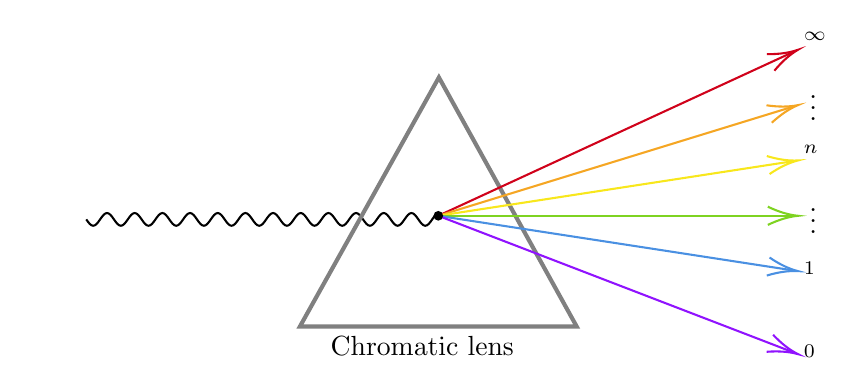
\begin{tikzpicture}[x=1pt,y=1pt,yscale=-1,xscale=1]
    %uncomment if require: \path (0,300); %set diagram left start at 0, and has height of 300

    %Shape: Wave [id:dp4206352155629708] 
    \draw   (192.8,151.3) .. controls (193.62,152.48) and (194.4,153.6) .. (195.3,153.6) .. controls (196.2,153.6) and (196.98,152.48) .. (197.8,151.3) .. controls (198.62,150.12) and (199.4,149) .. (200.3,149) .. controls (201.2,149) and (201.98,150.12) .. (202.8,151.3) .. controls (203.62,152.48) and (204.4,153.6) .. (205.3,153.6) .. controls (206.2,153.6) and (206.98,152.48) .. (207.8,151.3) .. controls (208.62,150.12) and (209.4,149) .. (210.3,149) .. controls (211.2,149) and (211.98,150.12) .. (212.8,151.3) .. controls (213.62,152.48) and (214.4,153.6) .. (215.3,153.6) .. controls (216.2,153.6) and (216.98,152.48) .. (217.8,151.3) .. controls (218.62,150.12) and (219.4,149) .. (220.3,149) .. controls (221.2,149) and (221.98,150.12) .. (222.8,151.3) .. controls (223.62,152.48) and (224.4,153.6) .. (225.3,153.6) .. controls (226.2,153.6) and (226.98,152.48) .. (227.8,151.3) .. controls (228.62,150.12) and (229.4,149) .. (230.3,149) .. controls (231.2,149) and (231.98,150.12) .. (232.8,151.3) .. controls (233.62,152.48) and (234.4,153.6) .. (235.3,153.6) .. controls (236.2,153.6) and (236.98,152.48) .. (237.8,151.3) .. controls (238.62,150.12) and (239.4,149) .. (240.3,149) .. controls (241.2,149) and (241.98,150.12) .. (242.8,151.3) .. controls (243.62,152.48) and (244.4,153.6) .. (245.3,153.6) .. controls (246.2,153.6) and (246.98,152.48) .. (247.8,151.3) .. controls (248.62,150.12) and (249.4,149) .. (250.3,149) .. controls (251.2,149) and (251.98,150.12) .. (252.8,151.3) .. controls (253.62,152.48) and (254.4,153.6) .. (255.3,153.6) .. controls (256.2,153.6) and (256.98,152.48) .. (257.8,151.3) .. controls (258.62,150.12) and (259.4,149) .. (260.3,149) .. controls (261.2,149) and (261.98,150.12) .. (262.8,151.3) .. controls (263.62,152.48) and (264.4,153.6) .. (265.3,153.6) .. controls (266.2,153.6) and (266.98,152.48) .. (267.8,151.3) .. controls (268.62,150.12) and (269.4,149) .. (270.3,149) .. controls (271.2,149) and (271.98,150.12) .. (272.8,151.3) .. controls (273.62,152.48) and (274.4,153.6) .. (275.3,153.6) .. controls (276.2,153.6) and (276.98,152.48) .. (277.8,151.3) .. controls (278.62,150.12) and (279.4,149) .. (280.3,149) .. controls (281.2,149) and (281.98,150.12) .. (282.8,151.3) .. controls (283.62,152.48) and (284.4,153.6) .. (285.3,153.6) .. controls (286.2,153.6) and (286.98,152.48) .. (287.8,151.3) .. controls (288.62,150.12) and (289.4,149) .. (290.3,149) .. controls (291.2,149) and (291.98,150.12) .. (292.8,151.3) .. controls (293.62,152.48) and (294.4,153.6) .. (295.3,153.6) .. controls (296.2,153.6) and (296.98,152.48) .. (297.8,151.3) .. controls (298.62,150.12) and (299.4,149) .. (300.3,149) .. controls (301.2,149) and (301.98,150.12) .. (302.8,151.3) .. controls (303.62,152.48) and (304.4,153.6) .. (305.3,153.6) .. controls (306.2,153.6) and (306.98,152.48) .. (307.8,151.3) .. controls (308.62,150.12) and (309.4,149) .. (310.3,149) .. controls (311.2,149) and (311.98,150.12) .. (312.8,151.3) .. controls (313.62,152.48) and (314.4,153.6) .. (315.3,153.6) .. controls (316.2,153.6) and (316.98,152.48) .. (317.8,151.3) .. controls (318.62,150.12) and (319.4,149) .. (320.3,149) .. controls (320.33,149) and (320.37,149) .. (320.4,149) ;

    %Shape: Triangle [id:dp28924046358844724] 
    \draw  [color={rgb, 255:red, 128; green, 128; blue, 128 }  ,draw opacity=1 ][line width=1.5]  (320.22,100) -- (370,190) -- (270,190) -- cycle ;

    %Straight Lines [id:da3725009850844284] 
    \draw [color={rgb, 255:red, 208; green, 2; blue, 27 }  ,draw opacity=1 ]   (320,150) -- (448.18,90.84) ;
    \draw [shift={(450,90)}, rotate = 155.22] [color={rgb, 255:red, 208; green, 2; blue, 27 }  ,draw opacity=1 ][line width=0.75]    (10.93,-3.29) .. controls (6.95,-1.4) and (3.31,-0.3) .. (0,0) .. controls (3.31,0.3) and (6.95,1.4) .. (10.93,3.29)   ;
    %Straight Lines [id:da04393101077336736] 
    \draw [color={rgb, 255:red, 245; green, 166; blue, 35 }  ,draw opacity=1 ]   (320,150) -- (448.09,110.59) ;
    \draw [shift={(450,110)}, rotate = 162.9] [color={rgb, 255:red, 245; green, 166; blue, 35 }  ,draw opacity=1 ][line width=0.75]    (10.93,-3.29) .. controls (6.95,-1.4) and (3.31,-0.3) .. (0,0) .. controls (3.31,0.3) and (6.95,1.4) .. (10.93,3.29)   ;
    %Straight Lines [id:da6751899671862938] 
    \draw [color={rgb, 255:red, 248; green, 231; blue, 28 }  ,draw opacity=1 ]   (320,150) -- (448.02,130.3) ;
    \draw [shift={(450,130)}, rotate = 171.25] [color={rgb, 255:red, 248; green, 231; blue, 28 }  ,draw opacity=1 ][line width=0.75]    (10.93,-3.29) .. controls (6.95,-1.4) and (3.31,-0.3) .. (0,0) .. controls (3.31,0.3) and (6.95,1.4) .. (10.93,3.29)   ;
    %Straight Lines [id:da7243327342564972] 
    \draw [color={rgb, 255:red, 126; green, 211; blue, 33 }  ,draw opacity=1 ]   (320,150) -- (448,150) ;
    \draw [shift={(450,150)}, rotate = 180] [color={rgb, 255:red, 126; green, 211; blue, 33 }  ,draw opacity=1 ][line width=0.75]    (10.93,-3.29) .. controls (6.95,-1.4) and (3.31,-0.3) .. (0,0) .. controls (3.31,0.3) and (6.95,1.4) .. (10.93,3.29)   ;
    %Straight Lines [id:da7878005985339279] 
    \draw [color={rgb, 255:red, 74; green, 144; blue, 226 }  ,draw opacity=1 ]   (320,150) -- (448.02,169.7) ;
    \draw [shift={(450,170)}, rotate = 188.75] [color={rgb, 255:red, 74; green, 144; blue, 226 }  ,draw opacity=1 ][line width=0.75]    (10.93,-3.29) .. controls (6.95,-1.4) and (3.31,-0.3) .. (0,0) .. controls (3.31,0.3) and (6.95,1.4) .. (10.93,3.29)   ;
    %Straight Lines [id:da4893685373249388] 
    \draw [color={rgb, 255:red, 144; green, 19; blue, 254 }  ,draw opacity=1 ]   (320,150) -- (448.13,199.28) ;
    \draw [shift={(450,200)}, rotate = 201.04] [color={rgb, 255:red, 144; green, 19; blue, 254 }  ,draw opacity=1 ][line width=0.75]    (10.93,-3.29) .. controls (6.95,-1.4) and (3.31,-0.3) .. (0,0) .. controls (3.31,0.3) and (6.95,1.4) .. (10.93,3.29)   ;
    %Straight Lines [id:da9572748849226034] 
    \draw    (320,150) ;
    \draw [shift={(320,150)}, rotate = 0] [color={rgb, 255:red, 0; green, 0; blue, 0 }  ][fill={rgb, 255:red, 0; green, 0; blue, 0 }  ][line width=0.75]      (0, 0) circle [x radius= 1.34, y radius= 1.34]   ;

    % Text Node
    \draw (280,192.4) node [anchor=north west][inner sep=0.75pt]   [align=left] {Chromatic lens};
    % Text Node
    \draw (172,145) node [anchor=north west][inner sep=0.75pt]    {$\Sp$};
    % Text Node
    \draw (451,195.4) node [anchor=north west][inner sep=0.75pt]    {$\C_{0}$};
    % Text Node
    \draw (451,82.4) node [anchor=north west][inner sep=0.75pt]    {$\C_{\infty }$};
    % Text Node
    \draw (451,165.4) node [anchor=north west][inner sep=0.75pt]    {$\C_{1}$};
    % Text Node
    \draw (451,123.4) node [anchor=north west][inner sep=0.75pt]    {$\C_{n}$};
    % Text Node
    \draw (453,99.4) node [anchor=north west][inner sep=0.75pt]    {$\vdots $};
    % Text Node
    \draw (453,140.4) node [anchor=north west][inner sep=0.75pt]    {$\vdots $};
    
    
    \end{tikzpicture}